\documentclass[10pt,a4paper]{article}

\usepackage[latin1]{inputenc}
\usepackage{amsmath}
\usepackage{amsfonts}
\usepackage{amssymb}
\usepackage{listings}
\usepackage{graphicx}
\title{Assignment No :A5}
\date{}


\begin{document}
\maketitle
\section{Title:}
Trigonometric calculator app.

\section{Problem Definition}
A mobile app for calculator having trigonometry functionality is to be designed and tested. The data storage uses :
\begin{itemize}
\item text files
\item XML
\end{itemize}
Use latest open source software modelling, designing and testing tool/Scrum-it. Implement the design using HTML-5/Scala/Python/Java/C++/Ruby on Rails. Perform positive and negative testing.

\section{Learning Objectives}
\begin{enumerate}
\item To understand mathematical and trigonometrical aspects of computer programs.
\item To understand android app management and building.
\item To perform problem analysis using the open source tools.
\end{enumerate}

\section{Learning Outcomes}
\begin{enumerate}
\item Ability to analyze problems and create meaningful user interfaces for them.
\item Acquired understanding of problem solving using practical implementation frameworks for transforming the algorithms into usable products.
\item Acquired knowledge about the documentation of typical software apps.
\end{enumerate}


\section{Related Mathematics}
Let S be the solution perspective of the given problem.\\
The set S is defined as:\\\\
$S=\lbrace\ s,e,X,Y,F,DD,NDD,S_{c},F_{c}|\varnothing_{s}\rbrace$ \\
Where,

s= Start state,  Such that $Y=\lbrace \varnothing \rbrace$ 

e= End state  \\\\
X= Input Set. \\\\
$X=\lbrace$ x = $\lbrace x \rbrace$ $\mid$ x $\in$ (Angle degrees) $\rbrace$ \\
Where,

Angle degrees $\in \lbrace$ 0 - 360 $\rbrace$ \\\\ 
Y=Output set.\\
$Y=\lbrace$ trigonometric results $\rbrace $ \\\\
F= Set of functions used.\\
F=$\lbrace sin(), cos(), tan(), sec(), cosec(), cot() \rbrace$ \\\\
sin() = function to calculate the sin value of given number\\
cos() = function to calculate the cos value of given number\\
tan() = function to calculate the tan value of given number\\
sec() = function to calculate the sec value of given number\\
cosec() = function to calculate the cosec value of given number\\
cot() = function to calculate the cot value of given number\\\\
DD=Deterministic data. \\
DD=
\begin{enumerate}
\item input numbers are proper (no hardware overflow).
\item numbers are proper degree values.
\item calculation terminates (the angles are finite)\\\\
\end{enumerate}
NDD= Non-deterministic data. \\
\\NDD= $\cup$ - DD\\


\section{State Transition diagram}
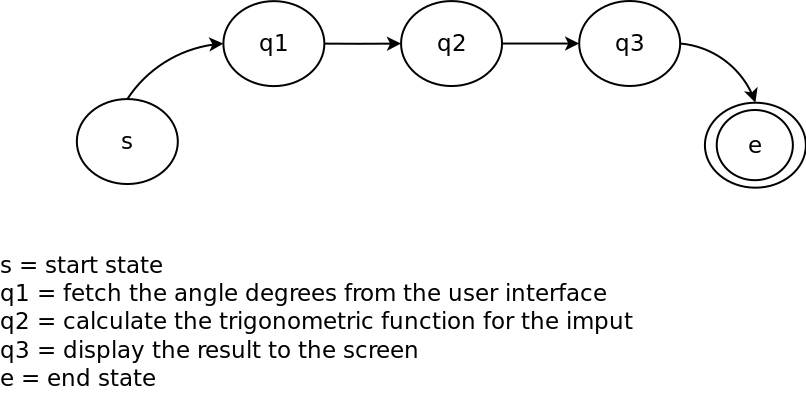
\includegraphics[scale=0.24]{stdg.png}


\section{Concepts related theory}
\begin{itemize}
\item \textbf{Mobile App:}\\
A mobile app is a software application developed specifically for use on small, wireless computing devices, such as smartphones and tablets, rather than desktop or laptop computers.Mobile apps are designed with consideration for the demands and constraints of the devices and also to take advantage of any specialized capabilities they have. A gaming app, for example, might take advantage of the iPhone's accelerometer. 

A native mobile app is a smartphone application that is coded in a specific programming language, such as Objective C for iOS and Java for Android operating systems. Native mobile apps provide fast performance and a high degree of reliability. They also have access to a phone's various devices, such as its camera and address book. In addition, users can use some apps without an Internet connection. However, this type of app is expensive to develop because it is tied to one type of operating system, forcing the company that creates the app to make duplicate versions that work on other platforms.
\end{itemize}

\begin{itemize}
\item \textbf{Android:}\\
Android is the name of the mobile operating system owned by American company; Google. It most commonly comes installed on a variety of smartphones and tablets from a host of manufacturers offering users access to Google's own services like Search, YouTube, Maps, Gmail and more.

This means you can easily look for information on the web, watch videos, search for directions and write emails on your phone, just as you would on your computer, but there's more to Android than these simple examples.

Android phones are highly customisable and as such can be altered to suit your tastes and needs; with wallpapers, themes and launchers which completely change the look of your device's interface. You can download applications to do all sorts of things like check your Facebook and Twitter feeds, manage your bank account, order pizza and play games. You can plan events on from your phone's calendar and see them on your computer or browse websites on your desktop and pick them up on your phone.

There are hundreds of thousands of apps and games available to download from the Google Play store (formerly the Android Market). There are camera apps that allow you to take pictures with artistic effects and music players which allow you to stream music from the web or create playlists. You can customise the appearance of your Android handset with a number of wallpapers based on pictures you've taken yourself or downloaded from the internet too.
\item \textbf{File storage:}
	\begin{itemize}
   \item \textbf{Text file storage:}\\\\
Basically every file is just a series of bytes one after the other. That is, numbers between 0 and 255. In order to facilitate the storage device they are on, a file might be spread out to several areas on that device. From our point of view, each file is just a series of bytes. In general every file is a binary file, but if the data in it contains only text (letter, numbers and other symbols one would use in writing, and if it consists of lines, then we consider it a text file.

A simple text file needs no additional metadata to assist the reader in interpretation, and therefore may contain no data at all, which is a case of zero byte file.\\
	\item \textbf{XML Storage:}\\
HTML pages are used to display data. Data is often stored inside HTML pages. With XML this data can now be stored in a separate XML file. This way you can concentrate on using HTML for formatting and display, and be sure that changes in the underlying data will not force changes to any of your HTML code.

XML data can also be stored inside HTML pages as "Data Islands". You can still concentrate on using HTML for formatting and displaying the data. 

In the real world, computer systems and databases contain data in incompatible formats. One of the most time consuming challenges for developers has been to exchange data between such systems over the Internet. Converting the data to XML can greatly reduce this complexity and create data that can be read by different types of applications.
	\begin{itemize}
	\item XML is a markup language.

    \item  XML is a tag based language like HTML.

    \item XML tags are not predefined like HTML.

    \item  You can define your own tags which is why it is called extensible language.

    \item XML tags are designed to be self descriptive.

     \item XML is W3C Recommendation for data storage and transport.
	\end{itemize}
	

	\end{itemize}
\end{itemize}

\newpage
\section{Object oriented modelling}
\begin{itemize}
\item \textbf{Class diagram:}
\begin{figure}[h!]
		\centering
		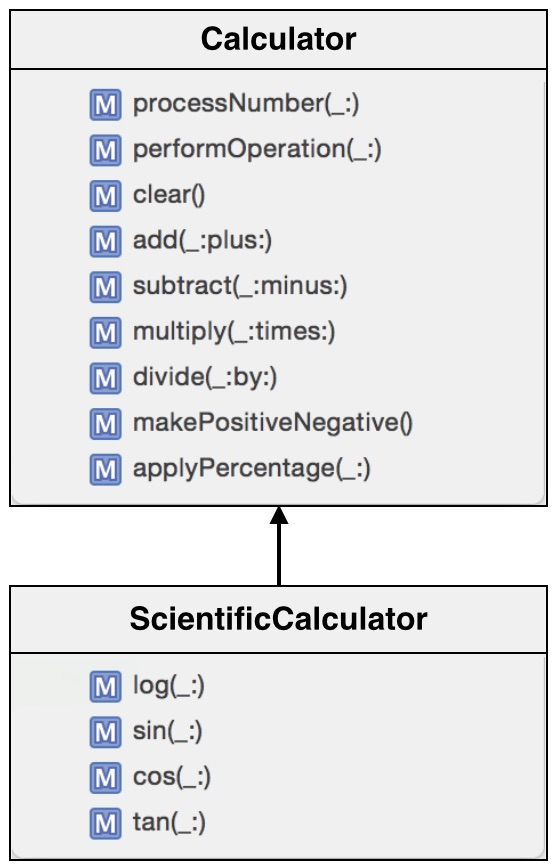
\includegraphics[scale=0.5]{Sci_Calc_class.jpg}
	\end{figure}

\newpage

\item \textbf{Use Case diagram :}

\begin{figure}[h!]
	\centering
	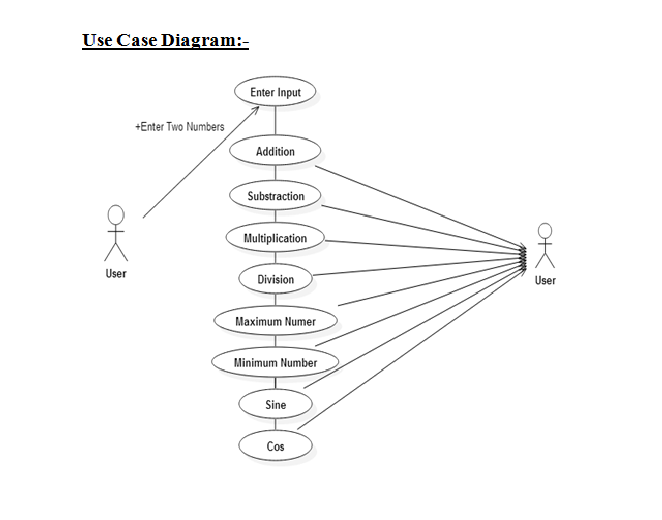
\includegraphics[scale=0.5]{usecase_calc.png}
\end{figure}

\item \textbf{Sequence diagram :}

\begin{figure}[h!]
	\centering
	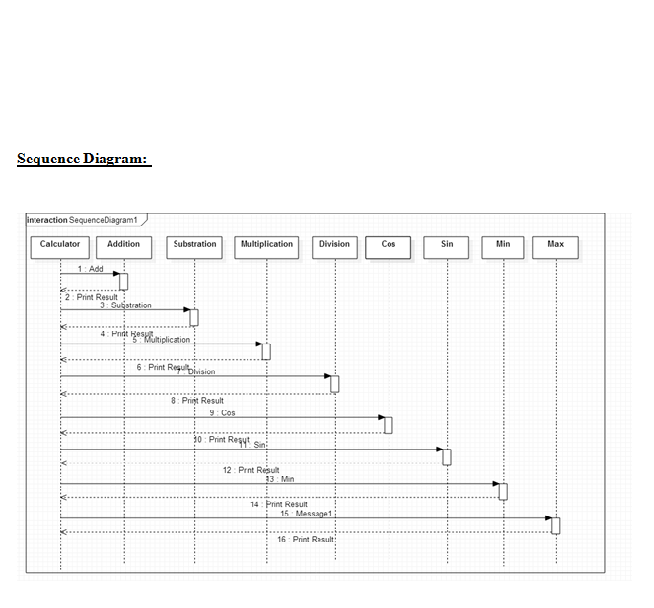
\includegraphics[scale=0.5]{seq_calc.png}
\end{figure}

\end{itemize}

\newpage
\section{Program Listing}
\begin{lstlisting}

// activity_main.xml

<?xml version="1.0" encoding="utf-8"?>
<RelativeLayout xmlns:android="http://schemas.android.com/apk/res/android"
    xmlns:tools="http://schemas.android.com/tools"
    android:layout_width="match_parent"
    android:layout_height="match_parent"
    android:paddingBottom="@dimen/activity_vertical_margin"
    android:paddingLeft="@dimen/activity_horizontal_margin"
    android:paddingRight="@dimen/activity_horizontal_margin"
    android:paddingTop="@dimen/activity_vertical_margin"
    tools:context="com.example.kiran.calculater.MainActivity">

    <GridView  xmlns:android="http://schemas.android.com/apk/res/android"
        android:layout_width="wrap_content"
        android:layout_height="wrap_content"
        android:numColumns="auto_fit"
        android:gravity="center"
        android:columnWidth="70dp"
        android:id="@+id/gridView"
        android:layout_below="@+id/txtresult"
        android:stretchMode="columnWidth" />


    <TextView
        android:layout_width="match_parent"
        android:layout_height="wrap_content"
        android:text="Result"
        android:id="@+id/txtresult"
        android:paddingBottom="20dp"/>
</RelativeLayout>


// MainActivity.java

package com.example.botman.calculater;

import android.content.SharedPreferences;
import android.os.Bundle;
import android.os.Environment;
import android.preference.PreferenceManager;
import android.support.v7.app.AppCompatActivity;
import android.view.View;
import android.widget.AdapterView;
import android.widget.ArrayAdapter;
import android.widget.EditText;
import android.widget.GridView;
import android.widget.TextView;
import android.widget.Toast;

import java.io.File;
import java.io.FileOutputStream;
import java.io.OutputStream;
import java.io.OutputStreamWriter;
import java.util.ArrayList;

public class MainActivity extends AppCompatActivity implements 
AdapterView.OnItemClickListener{

    EditText in;
    TextView tv;
    String re="0";
    File file;
    int trigpos;
    ArrayList<Double> number =  new ArrayList<Double>();
    ArrayList<Integer> operator = new ArrayList<Integer>();
    GridView gridview;
    static double result=0;
    int pos=-1;
    public static String[] numpad = new String[]
    {"7","8","9","/",
            "4","5","6","*",
            "1","2","3","+",
            "Recall","0","=",
            "sin","cos","tan","clear"};
    @Override
    protected void onCreate(Bundle savedInstanceState) {
        super.onCreate(savedInstanceState);
        setContentView(R.layout.activity_main);
        gridview = (GridView)findViewById(R.id.gridView);
       // in = (EditText)findViewById(R.id.editText);
        tv = (TextView)findViewById(R.id.txtresult);
        ArrayAdapter<String> adapter = new 
        ArrayAdapter<String>(this,android.R.layout.simple_list_item_1,numpad);
        gridview.setAdapter(adapter);
        gridview.setOnItemClickListener(this);
    }

    public void onItemClick(AdapterView<?> parent, View v,int 
		position, long id)
    {
        int temp1;
        String temp = ((TextView) v).getText().toString();
        if(position == 3 || position == 7 || position == 11 )
        {
            number.add(result);
            re="0";
            pos = position;
            operator.add(pos);
        }
        else if(position==12)
        {
            SharedPreferences sharedpreference1 = 
            PreferenceManager.getDefaultSharedPreferences(this);
            String getdatafrompreference = 
            sharedpreference1.getString("result","10");
            tv.setText(getdatafrompreference);
        }
        else if(position==18)
        {
            tv.setText("");
            result=0;
            re = "0";
            pos=-1;
            number=null;
            operator=null;
        }
        else if(position==15 || position==16||position==17)
        {
            trigpos = position;
            operator.add(trigpos);
        }
        else
        {
            if(position==14)
            {
                number.add(result);
                int j=0;
                result = number.get(0);
                double tempe = result /180.0*(22/7.0);
                if(trigpos==15)
                 {
                result = Math.sin(tempe);
                }
                else if(trigpos==16)
                {
                    result = Math.cos(tempe);
                }
                else if(trigpos==17){
                    result = Math.tan(tempe);
                }
                for(int i=1;i<number.size();i++)
                {
                    int op = operator.get(j);
                    j++;
                    if(op==11)
                    {
                        result = result + number.get(i);
                    }
                    else if(op==7)
                    {
                        result = result * number.get(i);
                    }
                    else if(op==3)
                    {
                        result = result / number.get(i);
                    }


                }

                String tr1 = Double.toString(result);
                tv.setText(tr1);
                /*try{
                    SharedPreferences sharedpreference = 
                    PreferenceManager.getDefaultSharedPreferences(this);
                    SharedPreferences.Editor editor = 
                    sharedpreference.edit();
                    editor.putString("result",tr1);
                    editor.commit();
                }catch(Exception e)
                {
                        Toast.makeText(this,"Error",Toast.LENGTH_LONG).show();
                }*/

                try{

                    file = new 
                    File(Environment.getExternalStorageDirectory(),
                    "result.txt");
                    OutputStream fileOutput = new 
                    FileOutputStream(file);

                    OutputStreamWriter outputStreamWriter = 
                    new OutputStreamWriter(fileOutput);
                    outputStreamWriter.append(tr1);
                    outputStreamWriter.close();
                    fileOutput.flush();
                    fileOutput.close();

                }catch(Exception e)
                {
                    Toast.makeText(this,"Error",Toast.LENGTH_LONG).show();
                }
            }
            else
            {
                //result = Integer.parseInt(temp);
                //String tr = Double.toString(result);
                re = re+temp;
                int temppp = Integer.parseInt(re);
                result = temppp;
                tv.setText(re);
            }
        }
    }
}


\end{lstlisting}

\section{Output}
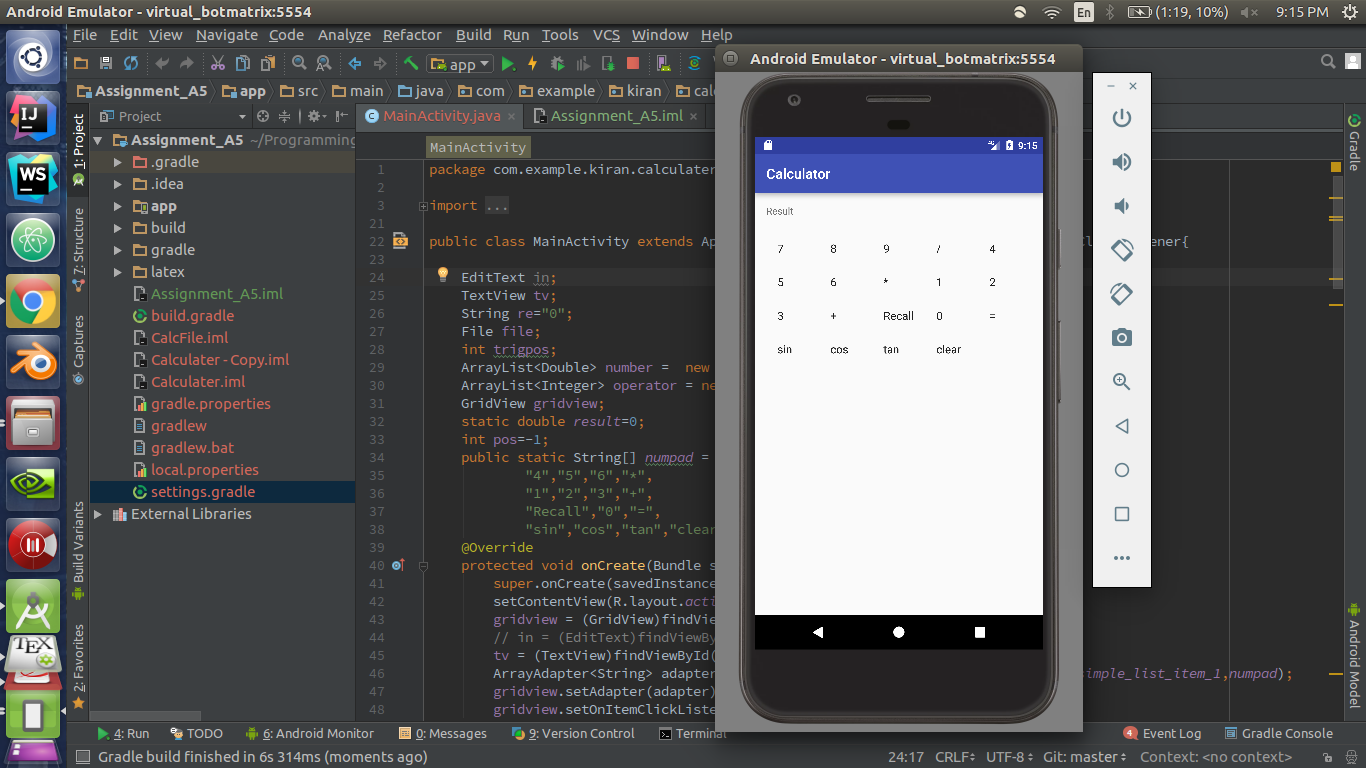
\includegraphics[scale=0.3]{out_1.png}

\section{Testing}
\begin{itemize}
\item \textbf{Positive Testing:}\\
Positive testing is a testing technique to show that a product or application under test does what it is supposed to do. Positive testing verifies how the application behaves for the positive set of data.

Positive Testing verifies if the application is Not showing error when it is not supposed to and showing error when it is supposed to.

The system will show the appropriate output when it is tested against correct mathematical values. For example, for trigonometric functions, the system will show appropriate output in floating point numbers. Also for basic mathematical operations like addition, subtraction, it will show appropriate output.\\
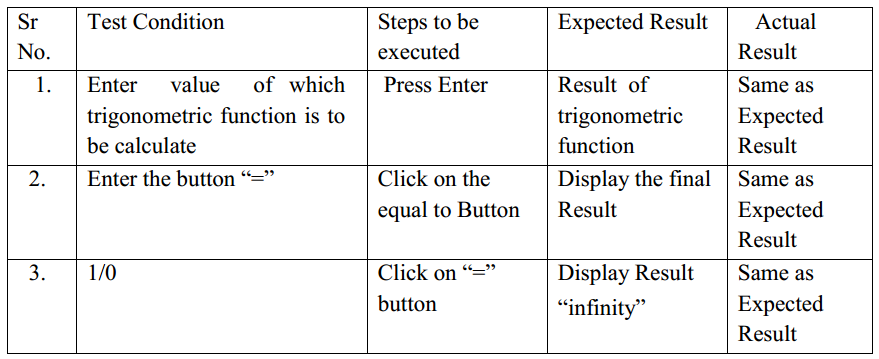
\includegraphics[width=\textwidth]{trig_positive}
\\

\item \textbf{Negative Testing:}\\
Negative testing is performed to ensure that the product or application under test does NOT fail when an unexpected input is given. The purpose of Negative testing is to break the system and to verify the application response during unintentional inputs.

Negative Testing is carried out to spot the faults that can result in significant failures.

Negative Testing is performed to expose the software weakness and potential for exploitation.

It is carried out to show data corruption or security breaches.

While performing the negative testing, the system will show incorrect output while performing the basic arithmetic operations if the user enters only a single number and performs addition without entering the second number. The system will give an error when the user attempts a divide by zero operation.\\
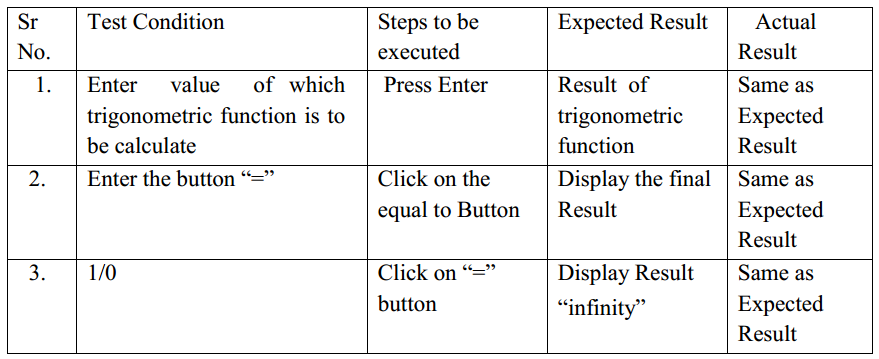
\includegraphics[width=\textwidth]{trig_positive}


\end{itemize}

\section{Conclusion}
We have studied and implemented an android application for the development of calculator app in android using java programming language and using storage in XML and text file.

\end{document}